\documentclass[tikz,border=8pt]{standalone}
\usepackage[T1]{fontenc}
\usepackage{helvet}\renewcommand{\familydefault}{\sfdefault}
\usepackage{amsmath}
\usetikzlibrary{arrows.meta,positioning,fit,calc,backgrounds}
\definecolor{tv}{HTML}{5F6B7A}\definecolor{tvf}{HTML}{EEF1F4}
\definecolor{dl}{HTML}{1F6FD0}\definecolor{dlf}{HTML}{E4EFFC}
\definecolor{pl}{HTML}{14875E}\definecolor{plf}{HTML}{E0F4EC}
\definecolor{pp}{HTML}{C8551B}\definecolor{ppf}{HTML}{FCEADF}
\begin{document}
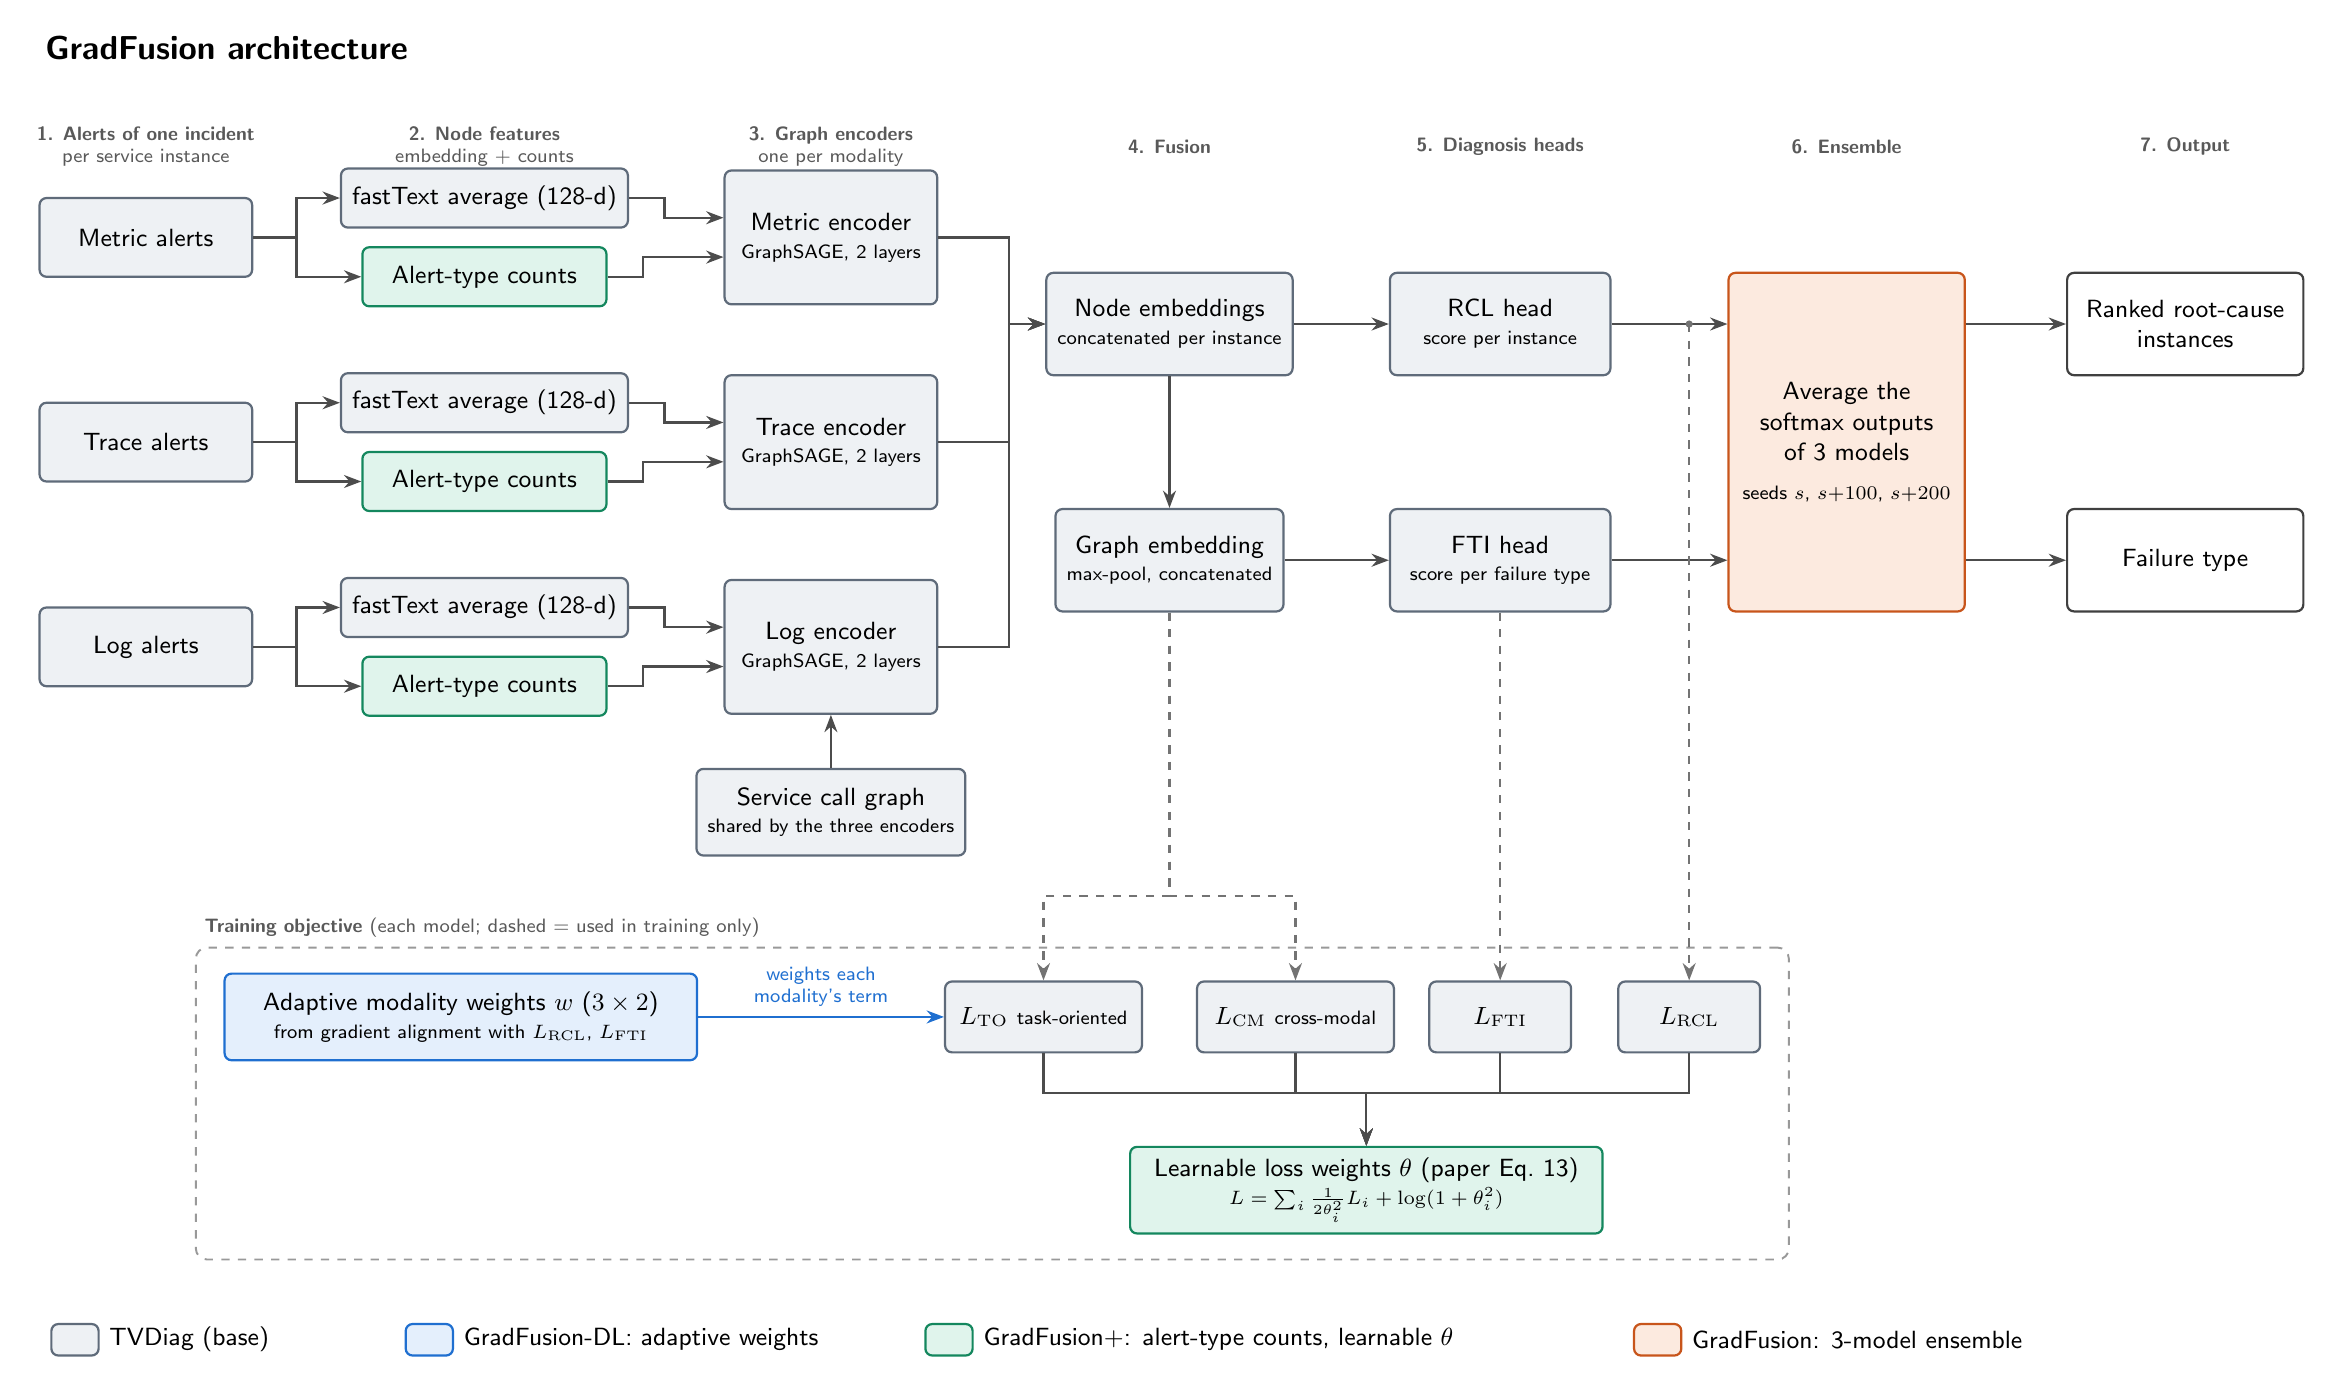
\begin{tikzpicture}[font=\small, >={Stealth[length=2.2mm]},
  box/.style={draw=#1, fill=#1f, rounded corners=2.5pt, line width=0.8pt, align=center,
              minimum height=10mm, inner sep=4pt},
  box/.default=tv,
  arr/.style={->, line width=0.8pt, draw=black!70},
  lab/.style={font=\scriptsize, text=black!65, align=center},
  grp/.style={draw=#1, dashed, rounded corners=4pt, line width=0.7pt, inner sep=7pt}]

% ---------- column 1: input
\node[box, minimum width=27mm] (met) at (0, 2.6) {Metric alerts};
\node[box, minimum width=27mm] (tra) at (0, 0)   {Trace alerts};
\node[box, minimum width=27mm] (log) at (0,-2.6) {Log alerts};
\node[lab] at (0, 3.75) {\textbf{1. Alerts of one incident}\\per service instance};

% ---------- column 2: features
\foreach \m/\y in {met/2.6, tra/0, log/-2.6}{
  \node[box, minimum width=31mm, minimum height=7.5mm] (e\m) at (4.3, \y+0.5) {fastText average (128-d)};
  \node[box=pl, minimum width=31mm, minimum height=7.5mm] (c\m) at (4.3, \y-0.5) {Alert-type counts};
  \draw[arr] (\m.east) -- ++(0.55,0) |- (e\m.west);
  \draw[arr] (\m.east) -- ++(0.55,0) |- (c\m.west);
}
\node[lab] at (4.3, 3.75) {\textbf{2. Node features}\\embedding + counts};

% ---------- column 3: encoders
\foreach \m/\y/\n in {met/2.6/Metric, tra/0/Trace, log/-2.6/Log}{
  \node[box, minimum width=27mm, minimum height=17mm] (g\m) at (8.7, \y) {\n\ encoder\\[-1pt]{\scriptsize GraphSAGE, 2 layers}};
  \draw[arr] (e\m.east) -- ++(0.45,0) |- ([yshift=2.5mm]g\m.west);
  \draw[arr] (c\m.east) -- ++(0.45,0) |- ([yshift=-2.5mm]g\m.west);
}
\node[lab] at (8.7, 3.75) {\textbf{3. Graph encoders}\\one per modality};
\node[box, minimum width=27mm, minimum height=11mm] (graph) at (8.7,-4.7) {Service call graph\\[-1pt]{\scriptsize shared by the three encoders}};
\draw[arr] (graph.north) -- (glog.south);

% ---------- column 4: fusion
\node[box, minimum width=27mm, minimum height=13mm] (node) at (13.0, 1.5) {Node embeddings\\[-1pt]{\scriptsize concatenated per instance}};
\node[box, minimum width=27mm, minimum height=13mm] (pool) at (13.0,-1.5) {Graph embedding\\[-1pt]{\scriptsize max-pool, concatenated}};
\foreach \m in {met,tra,log}{ \draw[arr] (g\m.east) -- ++(0.9,0) |- (node.west); }
\draw[arr] (node.south) -- (pool.north);
\node[lab] at (13.0, 3.75) {\textbf{4. Fusion}};

% ---------- column 5: heads
\node[box, minimum width=28mm, minimum height=13mm] (rcl) at (17.2, 1.5) {RCL head\\[-1pt]{\scriptsize score per instance}};
\node[box, minimum width=28mm, minimum height=13mm] (fti) at (17.2,-1.5) {FTI head\\[-1pt]{\scriptsize score per failure type}};
\draw[arr] (node.east) -- (rcl.west);
\draw[arr] (pool.east) -- (fti.west);
\node[lab] at (17.2, 3.75) {\textbf{5. Diagnosis heads}};

% ---------- column 6: ensemble + output
\node[box=pp, minimum width=30mm, minimum height=43mm] (ens) at (21.6, 0) {Average the\\softmax outputs\\of 3 models\\[3pt]{\scriptsize seeds $s$, $s{+}100$, $s{+}200$}};
\draw[arr] (rcl.east) -- (rcl.east -| ens.west);
\draw[arr] (fti.east) -- (fti.east -| ens.west);
\node[lab] at (21.6, 3.75) {\textbf{6. Ensemble}};
\node[box, draw=black!75, fill=white, minimum width=30mm, minimum height=13mm] (o1) at (25.9, 1.5) {Ranked root-cause\\instances};
\node[box, draw=black!75, fill=white, minimum width=30mm, minimum height=13mm] (o2) at (25.9,-1.5) {Failure type};
\draw[arr] (ens.east |- o1) -- (o1.west);
\draw[arr] (ens.east |- o2) -- (o2.west);
\node[lab] at (25.9, 3.75) {\textbf{7. Output}};

% ---------- training objective (bottom band)
\node[box, minimum width=25mm, minimum height=9mm] (lto)  at (11.4,-7.3) {$L_{\mathrm{TO}}$ {\scriptsize task-oriented}};
\node[box, minimum width=25mm, minimum height=9mm] (lcm)  at (14.6,-7.3) {$L_{\mathrm{CM}}$ {\scriptsize cross-modal}};
\node[box, minimum width=18mm, minimum height=9mm] (lfti) at (17.2,-7.3) {$L_{\mathrm{FTI}}$};
\node[box, minimum width=18mm, minimum height=9mm] (lrcl) at (19.6,-7.3) {$L_{\mathrm{RCL}}$};
\node[box=dl, minimum width=60mm, minimum height=11mm] (w) at (4.0,-7.3) {Adaptive modality weights $w$ ($3\times2$)\\[-1pt]{\scriptsize from gradient alignment with $L_{\mathrm{RCL}}$, $L_{\mathrm{FTI}}$}};
\node[box=pl, minimum width=60mm, minimum height=11mm] (theta) at (15.5,-9.5) {Learnable loss weights $\theta$ (paper Eq.~13)\\[-1pt]{\scriptsize $L=\sum_i \tfrac{1}{2\theta_i^2}L_i+\log(1+\theta_i^2)$}};
\draw[arr, draw=dl] (w.east) -- node[above, lab, text=dl]{weights each\\modality's term} (lto.west);
\foreach \l in {lrcl,lfti,lto,lcm}{ \draw[arr] (\l.south) -- ++(0,-0.5) -| (theta.north); }
\draw[arr, dashed, draw=black!55] (pool.south) -- ++(0,-3.6) -| (lto.north);
\draw[arr, dashed, draw=black!55] (pool.south) -- ++(0,-3.6) -| (lcm.north);
\draw[arr, dashed, draw=black!55] (fti.south) -- (lfti.north);
\draw[arr, dashed, draw=black!55] (19.6,1.5) -- (lrcl.north);
\fill[black!55] (19.6,1.5) circle (1.3pt);
\begin{scope}[on background layer]
  \node[grp=black!40, fit=(w)(lcm)(theta)(lrcl), inner xsep=10pt, inner ysep=9pt] (train) {};
\end{scope}
\node[lab, anchor=south west] at (train.north west) {\textbf{Training objective} (each model; dashed = used in training only)};

% ---------- legend
\node[box, minimum width=6mm, minimum height=4mm, inner sep=0] (k1) at (-0.9,-11.4) {};
\node[anchor=west] at (k1.east) {TVDiag (base)};
\node[box=dl, minimum width=6mm, minimum height=4mm, inner sep=0] (k2) at (3.6,-11.4) {};
\node[anchor=west] at (k2.east) {GradFusion-DL: adaptive weights};
\node[box=pl, minimum width=6mm, minimum height=4mm, inner sep=0] (k3) at (10.2,-11.4) {};
\node[anchor=west] at (k3.east) {GradFusion+: alert-type counts, learnable $\theta$};
\node[box=pp, minimum width=6mm, minimum height=4mm, inner sep=0] (k4) at (19.2,-11.4) {};
\node[anchor=west] at (k4.east) {GradFusion: 3-model ensemble};
\node[font=\large\bfseries, anchor=west] at (-1.4, 5.0) {GradFusion architecture};
\end{tikzpicture}
\end{document}
